\subsection{Experiments}

	To test the performance of the robot it was tested in a physical setup. On top of the modelled noise there was also considerable false ultrasonic sensor readings due to the low angle between the sensor ray and the walls, which made the navigation harder,see Figure \ref{fig:scan1}, and also the time required to make the movement made the whole process slower. 
	
	The time it takes to get to a random target point on the map is typically between 53-180s depending on the starting point. A simple signal conditioning.
	
		\begin{figure}[h]
			\centering
			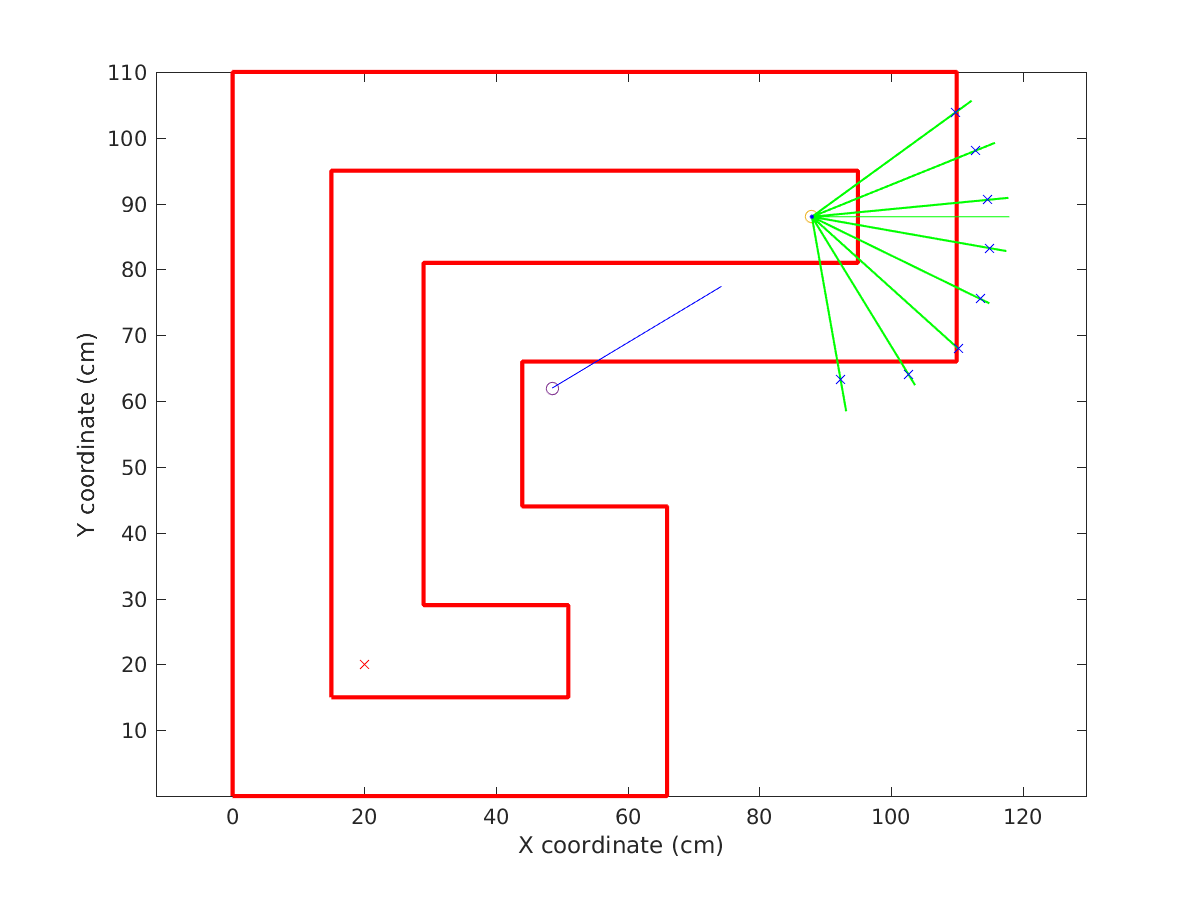
\includegraphics[width=\textwidth]{scan1}
			\caption{Sensor scanning beams showing the error between the perception of the robot and the map}
			\label{fig:scan1}
		\end{figure}
		